\chapter{\IfLanguageName{dutch}{Basisconfiguraties op de servers}{Introduction}}
\label{ch:basisconf}
In dit hoofdstuk wordt voor het eerst een onderzoek uitgevoerd. 

Er wordt voor elke server een configuratie bestand gemaakt dat 4 basisconfiguraties zal uitvoeren: gebruikers en groepen toevoegen, packages installeren en updates, mappen structuur aanmaken en ssh configuratie. 


\section{Aanmaken configuratie bestanden}
In dit hoofdstuk zal uitglegd worden hoe de playbooks en cloudconfig bestanden worden aangemaakt en opgesteld. 

Eerst wordt uitgelegd hoe de cloud-init configuraties worden gedaan, erna het Ansible playbook. Ten laatste zullen de set-ups worden gemaakt waar een combinatie wordt gebruikt.

De gebruiker die zal worden aangemaakt is \textit{bachelor} met wachtwoord \textit{proef}. De gebruiker zal behoren tot de groep \textit{test} die ook zal worden aangemaakt. De packages die zullen worden geïnstalleerd zijn: \textit{pwgen}, \textit{tree} en \textit{git}. De mappenstructuur die zal worden aangemaakt ziet er uit zoals die foto hieronder. En ten laatste zal er op de server een publieke ssh sleutel worden toegevoegd zodat er toegang is vanaf een test server. Figuur \ref{fig:mappen} is een visueel voorbeeld van de mappenstructuur.

\begin{figure}[!htb]
	\center{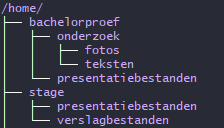
\includegraphics[width=0.45\textwidth]{img/mappenstructuur.png}}
	\caption{Mappen structuur basis configuraties.}
	\label{fig:mappen}
\end{figure}
\subsection{Opstellen cloud-init config bestand}
Als eerste zal het cloudconfig bestanden worden opgesteld. Dit bestand werd opgesteld met behulp van \autocite{clouddocs}.

Eerst werd er bekeken welke modules er nodig zullen zijn voor het opstellen van dit bestand. De modules \textit{packages} en \textit{package\_upgrade} zullen worden gebruikt voor de packages. De modules \textit{users} en \textit{groups} zullen worden gebruikt voor het toevoegen van gebruikers en groepen. 

Voor het toevoegen van de ssh sleutel, wordt de module \textit{ssh\_authorized\_keys} gebruikt. Hier worden de publieke sleutels die zijn toegelaten toegevoegd.

Voor het aanmaken van bestanden bestaat er de module \textit{write\_files}, spijtig genoeg is er geen module voor het aanmaken van mappen. Voor het aanmaken van de mappenstructuur werd dus de module \textit{runcmd} gebruikt.

\subsubsection{Packages}
Hierna werd het effectieve bestand gevormd. Onder de \textit{packages} werden de 3 packages opgelijst: \textit{git}, \textit{pwgen} en \textit{tree}. Bij \textit{package\_upgrade} werd \textit{true} gezet. 
\begin{lstlisting}[basicstyle=\small]
packages:
- pwgen
- git
- tree

package_upgrade: true
\end{lstlisting}

\subsubsection{Users \& Groups}
Bij \textit{groups} moest niet veel gedaan worden. Er werd gewoon de groepsnaam van de groep gezet.

Bij \textit{users} werden verschillende dingen ingevuld. Eerst en vooral de name, \textit{bachelor}. Bij groups de naam van de aangemaakte groep. Het wachtwoord onder passwd, proef, werd geëncrypteerd met de tool: \autocite{toolmkpass}. Als shell werd ook voor \textit{/bin/bash} gekozen.
\begin{lstlisting}[basicstyle=\small]
groups:
- test

users:
- default
- name: bachelor
- passwd: 985b56433efe9898290b88d4dab853a2f09d7eb7a7b1b8d2cdd431
- groups: test
- shell: /bin/bash
\end{lstlisting}


\subsubsection{Runcdm}
Bij de module \textit{runcmd} werden alle commando's gezet voor het aanmaken van de mappen structuur. Dit zijn gewoon 5 \textit{mdkir} commando's. Dit is het commando voor het aanmaken van mappen. Met de paramater \textit{-f} wordt heel de mappen structuur meegegeven aangemaakt als die er nog niet is.
\begin{lstlisting}[basicstyle=\small]
runcmd:
- mkdir /home/bachelorproef/onderzoek/fotos -f
- mkdir /home/bachelorproef/onderzoek/teksten -f
- mkdir /home/bachelorproef/presentatiebestanden -f
- mkdir /home/stage/presentatiebestanden -f
- mkdir /home/stage/veslagbestanden -f
\end{lstlisting}

\subsubsection{Ssh}
Als laatste wordt de ssh sleutel toegevoegd aan de server. Bij de waarde \textit{<insert key value>} wordt de publieke sleutel van de host die gaat connecteren gezet.
\begin{lstlisting}[basicstyle=\small]
ssh_authorized_keys:
- ssh-rsa <INSERT KEY VALUE>
\end{lstlisting}

Helemaal onderaan werd ook iets gezet onder de module \textit{final\_message}, namelijk: \textit{"The system is finally up, after \$UPTIME seconds"}. Door de waarde \textit{\$UPTIME} kan er gekeken worden hoelang de server nodig had om alles uit te voeren.

\subsection{Opstellen Ansible playbook}
Als tweede werd het Ansible playbook opgesteld. Als host wordt gekozen voor localhost. Aan het \textit{ansible.cfg} bestand werd ook nog de regel \textit{callback\_whitelist = profile\_tasks}. Zo kan er bekeken worden hoelang het draaien van het playbook duurde. Alle configuraties die worden gedaan werden in verschillende \textit{tasks} gezet. 

\subsubsection{Packages}
Voor het upgraden van de packages en installeren van de nodige packages werd de task \textit{apt} gebruikt.
\begin{lstlisting}[basicstyle=\small]
- name: Upgrade all packages to the latest version
apt:
name: "*"
state: latest
- name: Install git
apt:
name: git
state: present
- name: Install tree
apt:
name: tree
state: present
- name: Install pwgen
apt:
name: pwgen
state: present
\end{lstlisting}
\subsubsection{Mappen structuur}
Voor het aanmaken van de mappen structuur werd de task \textit{file} gebruikt. De state werd dan op directory gezet.
\begin{lstlisting}[basicstyle=\small]
- name: Creates direcory fotos
file:
path: /home/bachelorproef/onderzoek/fotos
state: directory
- name: Creates direcory teksten
file:
path: /home/bachelorproef/onderzoek/teksten
state: directory
- name: Creates direcory bachelor presentatie
file:
path: /home/bachelorproef/presentatiebestanden
state: directory
- name: Creates direcory stage presentatie
file:
path: /home/stage/presentatiebestanden
state: directory
- name: Creates direcory stage verslag
file:
path: /home/stage/verslagbestanden
state: directory
\end{lstlisting}
\subsubsection{Users \& groups}
Bij het aanmaken van de gebruikers en groepen werden de tasks \textit{group} en \textit{user} gebruikt. Bij de \textit{user} werden het shell en password meegeven. Ook de groups werden meegegeven.
\begin{lstlisting}[basicstyle=\small]
- name:  add group test
group:
name: test
state: present
- name:  add user bachelor
user:
name: bachelor
groups: test
shell: /bin/bash
password: 985b56433efe9898290b88d4dab853a2f09d7eb7a7b1b8d2cdd431e2920c35
\end{lstlisting}

\subsubsection{Ssh}
Voor het toevoegen van de ssh sleutel aan de server, zodat er een extra connectie kan worden gelegd, wordt de task \textit{authorized\_key} gebruikt. De user die wordt meegegeven is de bachelor user.
\begin{lstlisting}[basicstyle=\small]
- name: Set authorized key taken from file
authorized_key:
user: bachelor
state: present
key: ssh-rsa <INSERT KEY VALUE>

\end{lstlisting}

\subsection{Ansible \& cloud-init omgevingen}
Beide bestanden die apart gemaakt zijn, zijn vrij complexloos. Beide bestanden zijn vrij duidelijk. Wat als nadeel is voor het gebruik van een combinatie van Ansible en cloud-init. De enige uitvoering die complex is de bestanden is het aanmaken van de mappen via cloud-init. Dit is een beetje 'dirty' gedaan. Voor het werken met een combinatie gaat eerst alles via cloud-init worden gedaan. Het aanmaken van de mappen dan via Ansible.

\subsubsection{Verwijzing Ansible}
Voor de cloud setup wordt de verwijzing via github gedaan. Er wordt een git repository aangemaakt met het playbook in. Die wordt dan gecloned in cloud-init en uitgevoerd.

In cloud-init wordt drie modules toegevoegd: \textit{runcmd} en \textit{ssh\_keys}. In de module \textit{ssh\_keys} wordt de private sleutel toegevoegd connectie legt met de git repo. In de module \textit{runcmd} worden 3 commando's gezet: het toevoegen van github aan het known host bestand, de git clone en het uitvoeren van het playbook. Bij de packages wordt ook de package \textit{ansible} gezet.
\begin{lstlisting}[basicstyle=\small]
ssh_keys:
rsa_private: | <key>
runcmd:
- ssh-keyscan github.com >> /etc/ssh/ssh_known_hosts
- ssh-agent bash -c 'ssh-add /etc/ssh/ssh\_host\_rsa\_key; 
git clone <repo>'
- ansible-playbook -i, /home/ansible/playbook.yaml
\end{lstlisting}


\section{Uitvoering \& resultaten}
\subsection{Complexiteit}
\subsubsection{Overzichtelijkheid}
Eerst en vooral wordt er gekeken naar het de overzichtelijkheid van het playbook bestand en het cloudconfig bestand. Terwijl beide bestanden yaml bestanden zijn, zien ze er toch compleet anders uit. In het cloudconfig bestand is alles mooi onderverdeeld in verschillende modules, die de taken uitvoert. Terwijl bij het Ansible playbook alles opgesomd bij de tasks staat. Cloud-init is hierdoor veel overzichtelijker. Het is hierdoor ook makkelijker om het bestand te wijzigen. Bij het gebruik van de combinatie het playbook wel overzichtelijker doordat dit maar een paar taken heeft. In figuur \ref{fig:basisconf_layout} staan de layouts van het cloud-init en Ansibles bestand.
\begin{figure}[!htb]
    \centering
    {{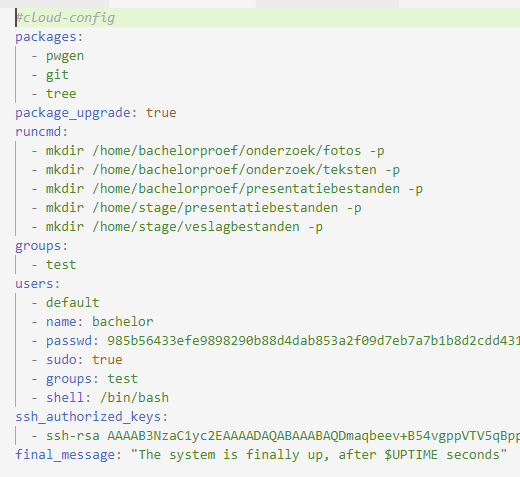
\includegraphics[width=0.45\textwidth]{img/basiscloud.png} }}%
    \qquad
    {{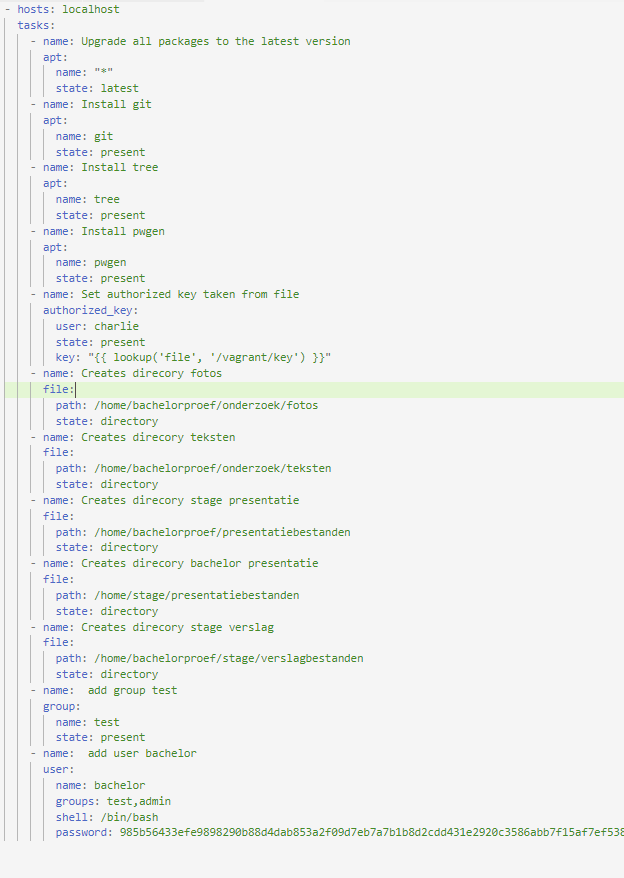
\includegraphics[width=0.45\textwidth]{img/basisansible.png} }}%
    \caption{Cloud-init en Ansible basis configuraties layout.}%
    \label{fig:basisconf_layout}%
\end{figure}
\subsubsection{Aanroepen uitvoeringen}
Ten tweede wordt er gekeken hoe alles werd aangeroepen. Voor het toevoegen van users, groepen en packages en het aanmaken van een nieuwe ssh sleutel zijn er voor Ansible en cloud-init aparte modules om dit te doen. Hier is weinig verschil. Maar voor het aanmaken van de mappen was er een verschil. Bij het toevoegen van de mappen is er bij Ansible een aparte module hiervoor. Terwijl bij cloud-init dit moest worden gedaan via runcmd en het \textit{mkdir} commando. 

Het aanroepen van de Ansible configuraties via cloud-init gebeurde via de commando module (\textit{runcmd}) in cloud-init. Dit gebeurde op een vrij efficiënte manier. Al moet er wel elke keer ene private sleutel van de repo worden meegegeven.

\subsection{Snelheid}
Als er puur naar de snelheid wordt gekeken is Ansible duidelijk sneller. Maar cloud-init heeft configuraties die het altijd uitvoert. Hierdoor kan deze statistiek soms misleidend. De gemiddelde uitvoersnelheid voor Ansible is 137.53 seconden en voor cloud-init is dit 177.77 seconden. Als er bij cloud-init het verschil van de startup configuraties wordt afgetrokken, komt dit eerder op 140-145 seconden. Dit ligt veel dichter bij Ansible, dit verschil is eigenlijk verwerpbaar. Al is Ansible een beetje sneller is dit niet zo een groot verschil dat dit een voordeel is voor Ansible. Er kan worden vastgesteld dat ze min of meer dezelfde uitvoeringssnelheid hebben.

De cloud-init en Ansible configuraties hebben bijna dezelfde uitvoeringssnelheid als cloud-init, namelijk 177.60 seconden. Net zoals bij cloud-init kan er hier worden afgerond naar 140-145 seconden door de eerste basisconfiguraties van cloud-init. Ook hier is dus weer geen groot verschil merkbaar.

In tabel \ref{tab:tabel resultaten basis} staan de resultaten van de snelheden.

\begin{table}[!htb]
    \centering
    \begin{tabular}{| l | l | l |l |}
        \hline
        \textbf{Uitvoeringstijd} & Resultaat 1 & Resultaat 2 & Resultaat 3   \\ \hline
        cloud-init & 179.75 sec & 187.74 sec & 165.51 sec  \\ \hline
        Anisble & 168.69 sec & 132.59 sec & 111.31 sec \\ \hline
        cloud-init \& Ansible & 149.10 sec & 190.13 sec & 193.59 sec \\
        \hline
    \end{tabular}
    \caption{Snelheid van Basisconfiguraties op de servers.}
    \label{tab:tabel resultaten basis}
\end{table}

\subsection{Resultaat}
Voor basisconfiguraties lijkt het meteen wel beter om dit niet met Ansible en cloud-init te doen. Dit lijkt iets te omslachtig voor het maar basis werk dat moet gebeuren. 

Voor Ansible en cloud-init apart is er niet zoveel verschil. Al is het cloudconfig bestand wel veel overzichtelijker, heeft Ansible iets meer variatie qua modules. Toch lijkt cloud-init in deze setup de beste optie. Het meegeven van het script gebeurt op een veer makkelijker manier. En doordat het maar basisconfiguraties zijn die hier worden getest, is het voordeel van de meer variatie van modules in Ansible nog niet zo doorslaggevend. De overzichtelijkheid van cloud-init is dat dan wel. Het bestand is veel compacter en veel duidelijker. Ook doordat het bestand op een makkelijkere manier kan worden uitgevoerd lijkt cloud-init hier de betere optie. Ansible geeft wel een betere output weer. Maar dit is hier nog niet doorslaggevend doordat er nog geen geavanceerde acties gebeuren.

Cloud-init lijkt, zeker als het in een gelijkaardige setup als deze gebeurt, de beste optie om eerste basisconfiguraties aan de server toe te voegen.
